关于执行模型,需要知道多少?近年来,并行内核作为一种表达数据并行性的方式出现。基于内核的方法主要设计目标是跨各种设备的可移植性,以便提高开发者工作效率。因此,内核通常不是硬编码处理特定数量或配置硬件资源(例如:内核、硬件线程、SIMD[单指令多数据]指令)。相反,内核用抽象的概念来描述并行性,实现(即编译器和运行时的组合)可以映射到特定目标设备上的可用硬件并行。尽管这种映射是由具体实现定义,但我们相信其会选择一种合理,且能够有效利用硬件并行性的映射。\par

以一种硬件无关的方式运行大量的并行计算,确保了应用程序可以扩展(或缩小)以适应不同平台的能力,但是……\par

\begin{tcolorbox}[colback=red!5!white,colframe=red!75!black]
保证功能的可移植性,但不保证高性能!
\end{tcolorbox}

支持的设备很多,不同的架构为不同的用例设计和优化。想要在特定的设备上达到最高的性能水平,总是需要一些手动优化工作——不管使用的是什么编程语言!这种特定于设备的优化的例子包括针对特定缓存大小的阻塞、选择平摊调度开销的粒度大小、使用专门的指令或硬件单元,以及最重要的是选择适当的算法。其中一些例子将在第15、16和17章中继续讨论。\par

应用程序开发过程中,在性能、可移植性和生产率之间的平衡是必须面对的一个挑战,也是本书不能完全解决的挑战。然而,我们希望证明DPC++提供了一种高级编程语言,可维护通用可移植代码和优化目标特定代码所需的所有工具。其余部分留给读者作为练习!\par

\hspace*{\fill} \par %插入空行
\textbf{多维内核}

许多语言的并行构造是1维的,直接将工作映射到1维硬件资源(例如:硬件线程数)。并行内核是一个更高层次的概念,它的维度更多地反映了代码要解决的问题(在1、2或3维空间中)。\par

为了开发者在1维空间开发方便,并行内核提供的多维索引。理解这个映射的行为方式可能是某些优化(例如:调优内存访问模式)的重要部分。\par

需要思考的是,哪个维度是连续的或“单位步幅”(即,多维空间中的数据落在一维空间中的位置)。SYCL中与并行性相关的多维变量都遵循相同的约定:维度从0到N-1进行编号。这种约定与标准C++中多维数组的行为一致。\par

SYCL将二维空间映射为线性索引的示例如图4-1所示。也可以打破这种方式,采用自己的方法来线性化索引,但这样做必须小心——打破惯例可能会对让步长为1访问方式有性能收益的设备产生负面的性能影响。\par

\hspace*{\fill} \par %插入空行
图4-1 映射二维范围(2,8)到线性索引上
\begin{center}
	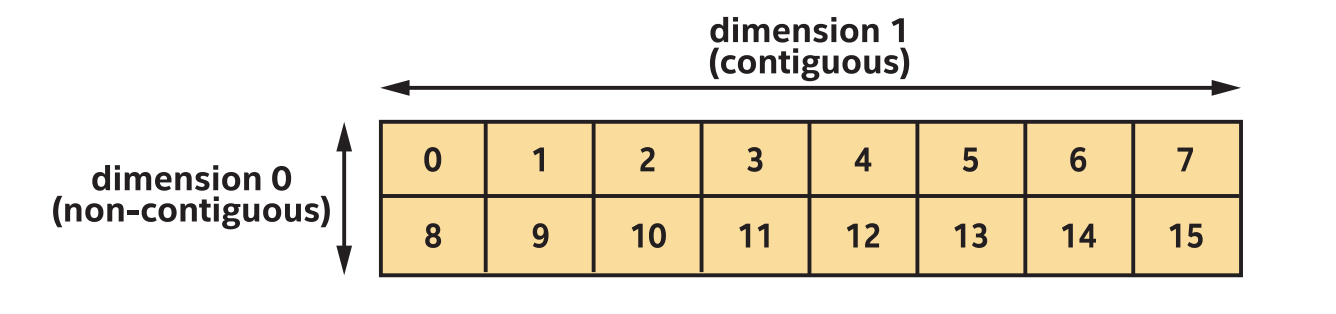
\includegraphics[width=1.\textwidth]{content/chapter-4/images/2}
\end{center}

如果程序需要大于三个维度,则必须使用模算法手动负责多维索引和线性索引之间的映射。\par

\hspace*{\fill} \par %插入空行
\textbf{循环与内核}

迭代循环是一种串行结构:循环的每次迭代都按顺序执行。优化的编译器可以确定迭代循环的部分或全部是否可以并行执行,但必须是保症,当编译器无法证明并行执行是安全的,则保持循环顺序语义的正确性。\par

\hspace*{\fill} \par %插入空行
图4-2 用串行循环表示向量加法
\begin{lstlisting}[caption={}]
for (int i = 0; i < N; ++i) {
	c[i] = a[i] + b[i];
}
\end{lstlisting}

考虑图4-2中的循环,描述了简单的向量加法。即使在这样的情况下,证明循环可以并行执行也不是一件简单的事情:只有当c不重叠a或b时,并行执行才是安全的。而在一般情况下,没有运行时检查是无法证明这一点的!为了解决这样的情况,语言添加了一些特性,使我们能够向编译器提供额外的信息,从而简化分析(例如,断言指针不与restrict重叠)或完全覆盖所有情况进行分析(例如,声明循环的所有迭代都是独立的,或者确切地定义应该如何将循环调度为并行资源)。\par

并行循环的含义有些含糊不清——因为不同的并行编程语言会重载这个术语——但是许多常见的并行循环构造表示,编译器转换顺序循环。这样的编程模型使我们能够编写顺序循环,并且只需要提供有关如何安全地并行执行不同迭代的信息。这些模型非常强大,与其他编译器优化集成得很好,并且极大地简化了并行编程,但这不代表鼓励开发者在开发的早期阶段就考虑并行性。\par

并行内核不是循环,也没有迭代。相反,一个内核表示一个操作,可以多次实例化,并应用于不同的输入数据;当一个内核并行启动时,该操作的多个实例将同时执行。\par

\hspace*{\fill} \par %插入空行
图4-3 将循环重写(伪代码)为并行内核代码
\begin{lstlisting}[caption={}]
launch N kernel instances {
	int id = get_instance_id(); // unique identifier in [0, N)
	c[id] = a[id] + b[id];
}
\end{lstlisting}

图4-3显示了使用伪代码重写为内核的简单循环示例。这个内核中实现并行性是明确的:内核可以由任意数量的实例并行执行,每个实例独立地应用于单独的数据块。通过将此操作编写为内核,可以确定并行运行是安全的(理想情况下应该如此)。\par

简而言之,基于内核的编程不是一种使用并行改进顺序代码的方法,而是一种编写显式并行程序的方法。\par

\begin{tcolorbox}[colback=red!5!white,colframe=red!75!black]
我们越早将思路从并行循环转向内核,就越容易使用Data parallel C++编写高效的并行程序。
\end{tcolorbox}
























